\documentclass[12pt]{article}

% set margins and spacing
\addtolength{\textwidth}{1.3in}
\addtolength{\oddsidemargin}{-.7in} %left margin
\addtolength{\evensidemargin}{-.7in}
\setlength{\textheight}{9in}
\setlength{\topmargin}{-.5in}
\setlength{\headheight}{0.0in}
\setlength{\footskip}{.375in}
\renewcommand{\baselinestretch}{1.0}
\linespread{1.0}

% load miscellaneous packages
\usepackage{csquotes}
\usepackage[american]{babel}
\usepackage[usenames,dvipsnames]{color}
\usepackage{graphicx,amsbsy,amssymb, amsmath, amsthm, MnSymbol,bbding,times, verbatim,bm,pifont,pdfsync,setspace,natbib}
\usepackage{float}

% enable hyperlinks and table of contents
\usepackage[pdftex,
bookmarks=true,
bookmarksnumbered=false,
pdfview=fitH,
bookmarksopen=true,hyperfootnotes=false]{hyperref}

% define environments
\newtheorem{definition}{Definition}
\newtheorem{fact}{Fact}
\newtheorem{result}{Result}
\newtheorem{proposition}{Proposition}



\begin{document}
\title{Shifting Revenue Strategy: The Inverse Relationship Between Consumption Tax and Tariff Revenue in Developed and Developing Countries}
\author{Umar Bilgrammi\thanks{Syracuse University, Email: ujbilgra@syr.edu} 
\and Dylan Thomas \thanks{Syracuse University, Email: dthoma26@syre.edu} 
\and Kathryn Sargge\thanks{Syracuse University, Email: kesarrge@syr.edu}
}

\date{\vskip-.1in \today}
\maketitle

\vskip.3in
\begin{center} {\bf Abstract} \end{center}

\begin{quote}
{\small We explore the relationship between consumption taxes, such as value added tax (VAT), and tariffs in developed and developing countries to better understand the revenue strategies employed by both groups of countries. Specifically, we explore the correlation between consumption tax and tariffs. We hypothesize that as revenue from consumption taxes increases, the profit from tariffs decreases, indicating a negative correlation between these two revenue variables. Using data from the World Integrated Trade Solution (WITS) database, which covers 194 countries from 1988 to 2022, we analyze consumption taxes and international taxes as a percentage of government revenue, considering their implications for economic development. Our findings reveal a moderate negative correlation between consumption tax and tariff revenue in developing and developed countries, with a correlation coefficient of -0.3255. The implications of this value indicate an inverse relationship between the two variables, which is further explored in the paper through findings from previous research papers, figures, and statistics, as well as databases and various reports on the subject. Our research synthesizes these findings with the broader literature on tax reform, analyzing the complex relationship between consumption taxes and tariffs.}
\end{quote}

\bigskip
\section{Introduction} \label{sec:introduction}
The generation of government revenues plays a vital role in shaping the long-term economic stability and growth of a country. As discussed by Michael et al. (1993), many countries rely on consumption taxes on goods and services, such as Value Added Tax (VAT), and tariffs on international trade as key sources of revenue. Furthermore, methods to generate revenue vary by country due to various factors including laws, border policies, and a country's economic strengths. Bird et. al (2008) explores the idea that a country's tax system is always constrained by what it can do, lending an explanation as to why methods to generate revenue by tax are so varied across the globe. Although both consumption tax and international tax are widely used around the world, our findings suggest an inverse relationship between consumption taxes and tariffs in developing and developed countries. Understanding the relationship between these two forms of taxation can offer valuable insights for policymakers aiming to optimize tax policies for national development and magnify revenue generation. By analyzing this relationship, we aim to provide critical insights into how governments can maximize their revenue sources. 

Based on the research question, "Is there an inverse relationship between VAT revenue and tariff revenue in developed and developing countries?", this study investigates the relationship between consumption tax and international taxes, in developed and developing countries. We hypothesize if a consumption tax such as VAT increases in a developed or developing country, then international taxes such as tariffs decrease. Our research question is not designed to investigate whether developed or developing countries have a specific preference towards consumption taxes or international taxes, but rather if there is an inverse correlation that is consistent between both sets of countries. We will examine data from the World Integrated Trade Solution (WITS) database. WITS is an aggregated database that collects economic data from multiple sources and combines it into easily accessible databases for analysis. Our WITS datasets provided information on both forms of taxation as a percentage of government revenue across 194 countries from 1988 to 2022. By analyzing these two key revenue sources, we hope to better understand the fiscal strategies employed by developing and developed nations with an emphasis on if revenue strategies are consistent with each other. 

In this paper, we will present a detailed analysis of the data collected from the WITS database, which includes consumption taxes, international taxes, and GDP per capita to help classify countries into developed or developing. We will start with a literature review that provides overall information on the current viewpoints regarding the relationship between consumption taxes and international taxes. Next, we will engage in a theoretical analysis using research papers to formulate a hypothesis and null hypothesis. Afterward, we will describe the data, along with its sources and variables. The results section will outline the relationship between these variables by providing a series of visualizations to illustrate the correlations found within the data. Using a P-value Test and Two Sample T-Test we will present statistical evidence against our null hypothesis. Finally, the paper will conclude with a discussion of the findings, their implications for developing and developed country's fiscal policy, and areas for further research.


\section{Literature Review} \label{sec:literature}

The literature on international and consumption taxes is extensive and highly saturated. Many studies cited in this research paper are recent from the years 2023 to 2024, while others date as far back as 1990. Michael Et. Al (1993) argues that reducing tariffs while increasing consumption taxes, can improve welfare and maintain or even enhance government revenue. The idea of reducing tariffs and increasing consumption taxes leads to an improvement in welfare as goods consumed within a country's borders will increase revenue streams for the government. 

Thuy Tien Ho, Xuan Hang Tran, and Quang Khai Nguyen (2023) investigate the link between tax revenue, economic growth, and trade openness, with a focus on developing countries. The paper finds that increased trade openness, facilitated by tariff reductions, can potentially support a shift to value added tax as a more stable source of revenue. Thus, the idea of a reduction in tariffs having positive effects on economic performance from Michael et. al (1993) is reinforced.  However, the paper mentions revenue challenges posed to developed and developing countries as a result of this shift which is explored in greater detail by Waglé et al (2011). This paper uses a set of data from the customs records of Nepal along with data from other countries similar to Nepal to reveal that many countries have mixed success when offsetting reductions in trade tax revenue and shifting to a value added tax model. This insight is important for understanding the complex and dynamic challenges that developed and developing countries face which hinder the benefits of reducing tariffs in favor of consumption taxes. Thus, the relationship between tariffs and consumption taxes seems to be intricately woven into politics, government structure, and relative income levels. 

The idea of consumption taxes being interwoven into politics is explored by Hansen et. al. (1990). In this paper, the idea of governments relying too heavily on one tax, either consumption tax or value added tax is explored, revealing a phenomenon called the “choke-off.” This occurs when the government relies on one tax too much, setting a rate too high or low, that it decreases collections and revenues. Thus, for some governments, it is within the realm of possibility that decreasing tariffs in favor of increasing consumption tax can decrease revenue and create an unsustainable reliance on value added tax. 

Furthermore, some readings provide insight into how countries use consumption tax and tariffs. According to Shahe Emran et. al. (2005), as countries become more developed, they rely less on tariffs and more on value added tax to generate revenue. This occurs due to the main idea that tariffs can impact consumers in harsher ways than value added tax can, causing countries to adjust to value added tax as they develop to increase revenue. Another process, called Trade Liberalization occurs when a country will decrease tariffs in an attempt to encourage international trade, increasing profit. This concept is explored in the International Monetary Fund (IMF) through an analysis of developing countries that engaged in Trade Liberalization. The paper analyzed a decrease in poverty, increases in jobs, and growth in GDP as a result of this concept as well.

The general consensus among researchers on the topic is that reducing tariffs and increasing consumption taxes can enhance revenue and welfare, but the success of these reforms depends on a variety of factors. Studies like those of Michael et al. (1993) and Thuy Tien Ho, Xuan Hang Tran, and Quang Khai Nguyen (2023) support the view that such reforms can be beneficial, while Hansen’s (1990) and Swarnim Waglé's 2011 paper juxtapose political economy with tariff reductions, highlighting the difficulties of overcoming tariff policies. Other readings such as Shahe Emran et. al. (2005) and Trade Liberalization from the IMF synthesize politics with tariff reductions, revealing that tariff reductions could in theory be offset by increasing value added tax. Furthermore, the readings analyze a variety of developed and developing countries, discussing the correlation between consumption taxes and tariffs which will be explored later in the paper as well. The highly nuanced and dynamic world of economics imposes different challenges for each country, creating volatility which makes it very difficult to conclusively state that reducing tariffs and increasing consumption tax always brings about positive effects for a country's economic development. While most studies support the idea that reducing tariffs and increasing VAT can improve revenue and welfare, they also highlight the importance of political will, effective enforcement, and addressing the informal economy. Our research builds on these findings by specifically examining the inverse relationship between VAT and tariff revenue, contributing to the ongoing discussion of tax reforms in developed and developing countries.


\section{Theoretical Analysis}
\label{sec:theory}
The relationship between consumption taxes and tariffs in opposition of one another. Tariffs represent the taxation of goods that are imported from other countries, while consumption tax represents domestic taxes on consumption of goods and services. Thus, the relationship between tariffs and consumption taxes can provide insight into a government's revenue structure. Generally, VAT is considered a more stable and efficient source of revenue than tariffs, especially as countries modernize their taxation, Kowalski, P. (2005). Tariffs, which are taxes imposed on imports, are often seen as a tool to protect domestic industries but can be disruptive to trade and economic efficiency, Michael et. al. (1993). This is because higher taxation discourages international trade from occurring, creating more room for domestic growth in production. As countries develop, it is expected that they may shift from relying on tariffs to more consumption-based taxes like VAT for improved revenue generation stability. Kowalski, P. (2005).

We hypothesize that there is a negative correlation between consumption taxes and tariff revenue in both developed and developing countries, based on our findings in the readings, and the research question. Therefore, our null hypothesis is that increases in consumption taxes do not affect tariffs in developed or developing countries. This hypothesis is grounded in the theory of tax modernization, where governments gradually move away from potentially risky taxes like tariffs and towards more efficient taxes like VAT. Kowalski, P. (2005). By examining this relationship, we aim to provide a more accurate view of revenue taxation in developing and developed countries.

\section{Data}
\label{sec:data}

We analyzed three time series data sources from the \href{https://wits.worldbank.org/CountryProfile/en/Country/BY-COUNTRY/StartYear/1988/EndYear/2022/Indicator/GC-TAX-GSRV-VA-ZS}{World Integrated Trade Solution} website, which provides detailed information about consumption taxes and tariffs as a percentage of revenue for developing and developed countries. By breaking down tariffs and consumption taxes in terms of percent of revenue, it is easier to observe how much revenue is generated from these taxes, and if they are growing year on year. We utilized a third variable, GDP per capita, which split countries into developed and developing depending on a cutoff value of 12,000 dollars which is derived from the United Nations "World Economic Situation and Prospects 2021" report, and Freed, Jeffrey S, et. al. (2020). The variables in our study are consumption tax, international tax, and GDP per capita. The international tax variable correlates to tariffs which were mentioned above in the literature review and theoretical analysis section. The data for the variables span from 1988 to 2022 and covers 194 countries. 

The WITS database aggregates data from various sources. It primarily compiles national statistics on tariffs and taxes from government reports and international organizations. The data collection process involves gathering information directly from the national governments' reports, which are often based on their domestic economic activities, tax laws, and trade statistics. The \href{https://wits.worldbank.org/CountryProfile/en/Country/BY-COUNTRY/StartYear/1988/EndYear/2022/Indicator/GC-TAX-GSRV-VA-ZS}{World Integrated Trade Solution} website provides more information on how they compile their database.

While the WITS dataset provides information for most countries, certain nations may have incomplete or missing data for specific years. In these cases, either the data is unavailable for that particular year or there are gaps due to inconsistencies in national reporting. For some countries, the data may not start until a later year, and for others, the data may be missing intermittently across the 34-year period. For example, Pakistan has entries for all three variables in consumption tax, international tax, and GDP per capita up until 2001, and then only has entries for GDP per Capita until the end of the dataset. Sri Lanka, a country in South Asia along with Pakistan has entries for all three variables for almost all years. The amount of countries that do not have entries at the start of the period or have no entries during certain periods called holes, is nearly split even. Upon dropping all variables that do not have a value, 2733 observations are left. Of these 2,733 observations, the large majority are developing countries, seemingly showing that the phenomena does differ by development status. This is most likely due to WITS sourcing a large portion of its data from a database called the UN Comtrade. According to WITS, ``The availability of the international trade statistics of UN Comtrade (The United Nations Commodity Trade Statistics database) via the WITS application has been made possible with the permission of the United Nations. UN Comtrade contains annual imports and exports statistics for more than 160 reporting countries or areas, which account for almost all trade worldwide. The trade statistics are detailed giving value and quantity for each commodity broken down by trading partner." Since WITS aggregates various database sources together to create it's databases, some data entries may not encompass all countries, leading to some of the gaps mentioned above. Furthermore, the UN Comtrade is known to have a significant amount of developing country data, meaning that when WITS aggregates it's databases, it is most likely pulling in more data from developing countries than developed countries. While this does not affect every entry, it may explain why some entries are blank within the data sets, especially for developed countries. Due to this, we only chose to remove bad data entries from our datasets and leave any other entries blank, since they would not count in the statistical tests. 

We acknowledge that the dataset is limited to the data available from the WITS platform, and some countries may have more reliable, consistent reporting than others. For example, it is easy to assume that developed countries often have more accurate and complete records, while developing countries may face challenges in data collection or reporting, but the analysis from WITS has shown the opposite, where developing countries have a more completed record of consumption tax, international tax, and GDP per capita than developed countries did. 

The collection of this data is subject to the availability and reliability of national statistical offices, and differences may arise depending on the country’s data reporting practices. A \href{https://taxsummaries.pwc.com/quick-charts/value-added-tax-vat-rates}{report} provided by Price-WaterHouse Coopers (PwC), a top global consulting firm shows the differences in Value Added Tax rates and how it is reported globally. Most notably, Brazil, Ghana, and India report Value Added Tax through three unique approaches. Brazil imposes three levels of value added tax from the federal, state and municipal level, which are between 5-30\%, 17-20\%, and 2-5\%, respectively. Ghana imposes value added tax through a standard rate scheme 15\%, flat rate scheme 3\%, and immovable property 5\%, with additional value added tax on tax applicable supplies. India levies value added tax between 5\% to 28\% depending on the good or service being supplied. Thus, data reporting of Value Added Tax is extremely varied depending on the political structure and a countries interpretation of what counts as value added tax. Value Added Tax reporting is extremely varied due to the lack of a centralized reporting system which other forms of taxation have. For example, Tariffs are relatively easy to report due to the Harmonized System developed by the World Customs Organization. Through the Harmonized System, every good is given a code that countries can then use to impose tariffs and disclose them to one another. For example, HS code:0702.00 refers to tomatoes that are either fresh or chilled. The United States reports its tariffs on goods through the \href{https://hts.usitc.gov/}{Harmonized Tariff Schedule}. The Harmonized Tariff Schedule reveals specific details behind the trading rules, regulations, and methodologies the United States uses when it imposes tariffs. Furthermore, the Harmonized Tariff Schedule outlines trading rules between the United States and various other countries including but not limited to Singapore, Oman, and Peru. In conclusion, reporting Value Added Tax is much less standardized than tariffs leading to more entries for tariffs in datasets than value added tax entries, although not by a significant amount.

The variables we use in our data are consumption tax, taxes on international trade, and GDP per capita. Consumption tax as a percent of revenue represents the tax revenue from value added tax or sales taxes divided by total revenue generated. It includes taxes levied on consumption, which can vary greatly across countries as observed in the PwC chart. Taxes on international trade as a percentage of revenue represents the revenue from tariffs divided by total revenue, providing insight into what value tariffs contribute to overall revenue. Finally, GDP per capita represents a country's gross domestic product divided by its population, which is considered an important indicator of the standard of living in a country. In our project specifically, GDP per capita will be used to identify developing and developed countries. Country's that are developed will have a GDP per capita of greater than 12,000 current USD. Countries that are developing have a GDP per capita that is less than or equal to 12,000 current USD based on the paper "Which Country Is Truly Developed? Covid-19 Has Answered the Question" (Freed, Jeffrey S, et al, 2020), and the "World Economic Situation and Prospects 2021" report by the United Nations. For our research, countries are evaluated on a year-by-year basis, therefore a country may be considered developing or developed depending on the year. 


\section{Results}
\label{sec:result}

In this section, we present an analysis of the relationship between taxes on consumption and international tax (tariffs) in developed and developing countries. Our primary focus is to investigate the potential inverse relationship between VAT revenue and tariff revenue, and to understand the trends over time. We also want to see if both developing and developed countries have an inverse correlation in consumption tax and tariffs. Firstly, we will look at descriptive statistics for all three variables, followed by graphs which provide insight and visualization to the trends and patterns within our data.

The summary statistics for all three variables in both developed and developing countries are presented in the table below.  

\begin{table}[h!]
\centering
\caption{Summary Statistics}
\label{tab:summary_stats}
\begin{tabular}{lrrrrr}
\hline
\textbf{Variable} & \textbf{Obs} & \textbf{Mean} & \textbf{Std. Dev.} & \textbf{Min} & \textbf{Max} \\
\hline
gdp              & 6,499        & 11,320.32     & 17,465.2           & 22.85037     & 133,590.1    \\
consumption      & 3,211        & 10.25779      & 5.280867           & 0.0329885    & 40.00499     \\
international& 2,969        & 10.24049      & 11.61363           & -0.1304207   & 64.65984     \\
\hline
\end{tabular}
\end{table}

Table 1 provides summary statistics for our three variables. Both international tax and consumption tax are expressed as percentages of total revenue, while GDP is measured in current (2024) U.S. dollars. The mean for both international tax and consumption tax is strikingly similar, at approximately 10.24 percent and 10.26 percent, respectively. While this table is informative for explaining the overall summary statistics of the dataset, more data can be discovered by creating summary statistics separately for developed and developing countries. 

\begin{table}[h!]
\centering
\caption{Summary Statistics for Developing Countries}
\label{tab:summary_stats}
\begin{tabular}{lrrrrr}
\hline
\textbf{Variable} & \textbf{Obs} & \textbf{Mean} & \textbf{Std. Dev.} & \textbf{Min} & \textbf{Max} \\
\hline
gdp              & 4,713        & 2,991.54      & 2,907.46           & 22.85037     & 1998.18      \\
consumption      & 2,111        & 9.553         & 4.88496            & 0.05734      & 2.11375      \\
international    & 2,228        & 12.37055      & 11.66786           & -0.00999     & 4.65984      \\
\hline
\end{tabular}
\end{table}
Table 2 provides us with summary statistics for developing countries only. The table contains a total of 4339 observations for the variables consumption and international from 194 countries in the years 1988 - 2022. It contains only entries for developing countries. In this table, consumption tax decreases from 10.25 percent in Table 1 to 9.5 percent. This shows that the mean for consumption taxes for developing countries is lower than the overall dataset.  International tax increases from 10.24 percent to 12.37 percent. This reveals that the mean for international tax in developing countries is higher than the overall dataset. 


\begin{table}[h!]
\centering
\caption{Summary Statistics for Developed Countries}
\label{tab:summary_stats}
\begin{tabular}{lrrrrr}
\hline
\textbf{Variable} & \textbf{Obs} & \textbf{Mean} & \textbf{Std. Dev.} & \textbf{Min} & \textbf{Max} \\
\hline
gdp              & 1,786        & 33,298.8      & 20,533.59          & 12,020.02    & 133,590.1    \\
consumption      & 1,100        & 11.61037      & 5.731912           & 0.0329885    & 40.00499     \\
international    & 741          & 3.835927      & 8.747825           & -0.1304207   & 58.70603     \\
\hline
\end{tabular}
\end{table}

Table 3 provides us with summary statistics for developed countries. There is a total of 1,841 observations for the variables consumption and international. These observations are from 194 countries from the year 1988 to 2022 and include developing countries only. The amount of observations for developed countries is significantly lower due to WITS sourcing a large portion of data from the UN Comtrade, which reports more data on developing countries than developed. In this table, consumption tax increases from 10.25 percent in Table 1 to 11.61 percent. This shows that the mean for consumption taxes for developed countries is higher than the overall dataset.  International tax drops from 10.24 percent to 3.83 percent. This reveals that the mean for international tax in developed countries is lower than the overall dataset. 

Completing further analysis, it appears that the mean for consumption tax is higher in developed countries than in developing countries. The mean for international tax is higher in developing countries than in developed countries. Thus, the means for consumption tax and international tax are opposite of each other depending on if the country is developing or developed. 


Next, we will analyze histograms and scatter-plots to visualize the patterns in the data with an emphasis on the relationship it reveals between taxes and tariffs. 

\begin{figure}[H]
    \centering
    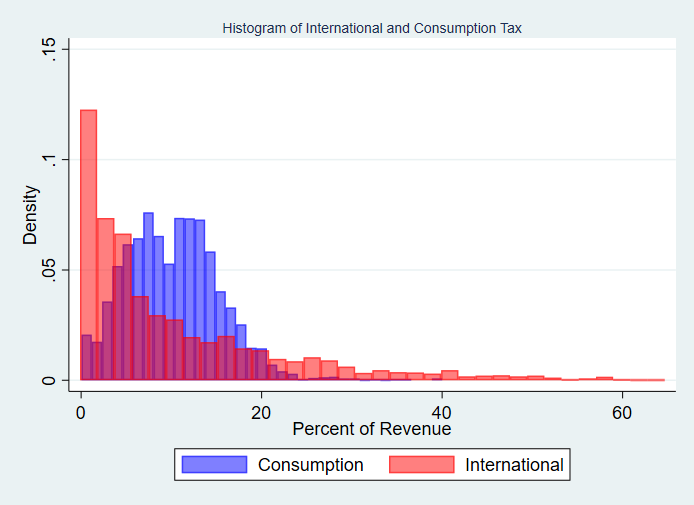
\includegraphics[width=0.8\linewidth]{Reproducibility_Package//research_outputs/twowayhistintcons.png}
    \caption{Histogram of International and Consumption Tax in Developed and Developing Countries}
    \label{fig:enter-label}
\end{figure}

Figure 1 provides a visualization that compares international and consumption tax in both Developed and Developing Countries. The X-axis represents the percent of revenue that consumption tax and international tax make up while the Y-axis is is called density because it essentially measures the concentration of entries in each percent of revenue from 0 to 70.The data includes information from 194 countries from 1988 to 2022, with a total of 6,180 observations. 

International tax is spread between 0 percent to 70 percent of revenue while Consumption tax has a lower spread in terms of percent of revenue, which is the X-axis of the graph. International tax has it’s highest density of entries at a lower percent of revenue, namely 0 to 5 percent. When compared to the density of consumption tax, the densities are different. Consumption tax has it’s highest density at around 10 percent of revenue, having a shape that resembles a normal distribution bell-shaped curve with a few dips at 10-11 percent of revenue. International tax seems to be right skewed due to the tail of values towards the right from around 30 to 60 percent of revenue. 

To provide further analysis on the intriguing relationship between the variables, we will now analyze two way histograms for the variables in developed and developing countries separately.
\begin{figure}[H]
    \centering
    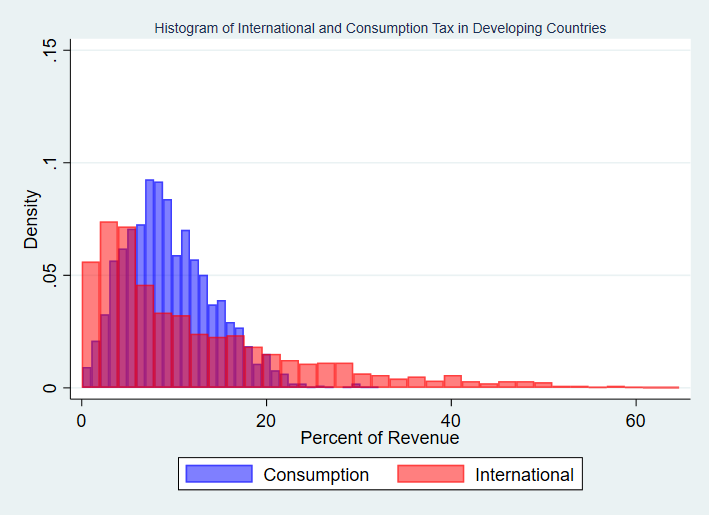
\includegraphics[width=0.8\linewidth]{Reproducibility_Package//research_outputs/twowaydevelopinghistintcons.png}
    \caption{Histogram of International and Consumption Tax in Developing Countries}
    \label{fig:enter-label}
\end{figure}

Figure 2 shows a histogram of International and Consumption tax in developing countries, allowing for a comparison of the variables with the main dataset which includes developed countries. This figure contains 4339 observations for the variables consumption and international from 194 countries for the years 1988 - 2022.  It must be noted that this histogram looks very similar to Figure 1, likely due to WITS having more data for developing countries than developed countries due to some of the sourcing of their data as mentioned in the Data Section. The most notable change in the graphs is the dip in density for international tax from around 0-5 percent of revenue. This is most likely because developing countries do not source a lot of revenue from tariffs as discussed by Michael et. al (1993), Ho et. al (2023). This means their data was removed from the density early on in the graph, leading to the drop in density observed above. The changes now accurately reflect how many developing countries get their revenue from tariffs with density decreasing at the start and spreading out, representing how developing countries do source more of their revenue from tariffs also discussed by Shahe Emran et. al (2005). Furthermore, consumption tax takes on more of a normal distribution compared to the graph above, resembling a bell-shaped curve. The change to a more normal bell-shaped curve is also due to the omittance of developed countries which source more of their revenues from value added tax and other forms of consumption tax, which would have had a significant effect on the data as observed in Figure 1, where there is an abnormally shaped normal distribution at the mean value of 10-11 percent of revenue. 

\begin{figure}[H]
    \centering
    \includegraphics[width=0.8\linewidth]{Reproducibility_Package//research_outputs/twowayhistdevelopedintcons.png}
    \caption{Histogram of International and Consumption Tax in Developed Countries}
    \label{fig:enter-label}
\end{figure}

Figure 3 displays the opposite relationship in comparison to Figure 2. International tax has a higher density in developed countries at lower percentages of revenue in Figure 4, while Figure 3 shows that International has a lower density in developing countries at higher percentages of revenue. This is most likely due to the recurring idea that developed countries are sourcing their revenue from value-added tax while developing countries source revenues from tariffs. Consumption tax changes back to its uneven bell-shape reflecting the various ways developed countries source their value added tax rates, as described by the PwC tables on value added tax in the data section. 

Exploring the histograms enabled us to visualize the data, providing insights into the behaviors of developed and developing countries with regard to taxes or tariffs preferences. 
For example, the summary statistics show that the mean for international tax is higher in developing countries, explaining why the histogram has more distribution compared to the general histogram. The more distribution creates a higher spread which increases the mean since the data is not as concentrated from 0 to 5 percent. Furthermore, this aligns with the findings in Michael et. al (1993), Ho et. al (2023) which discuss why developing countries rely more heavily on tariffs to generate revenue. On the other hand, consumption tax is not so easily explained due to two main reasons. The mean for consumption tax is higher in developed countries, aligning with the Michael et. al (1993), Ho et. al (2023) readings, however, the data has far less entries due to WITS sourcing of data from UN Comtrade, which mainly provides data on developing countries. Furthermore, the distribution of consumption tax is uneven as a result of the unstandardized methods to report value added tax globally. 

To determine if a correlation truly exists, we must analyze a scatterplot, conduct a P-Value Test, and a Two-Sample T-Test to be sure. 

We will now not analyze a scatterplot that provides correlation values between the two variables, allowing us to examine if there truly is an inverse relationship as stated in the project hypothesis. 

\begin{figure}[H]
    \centering
    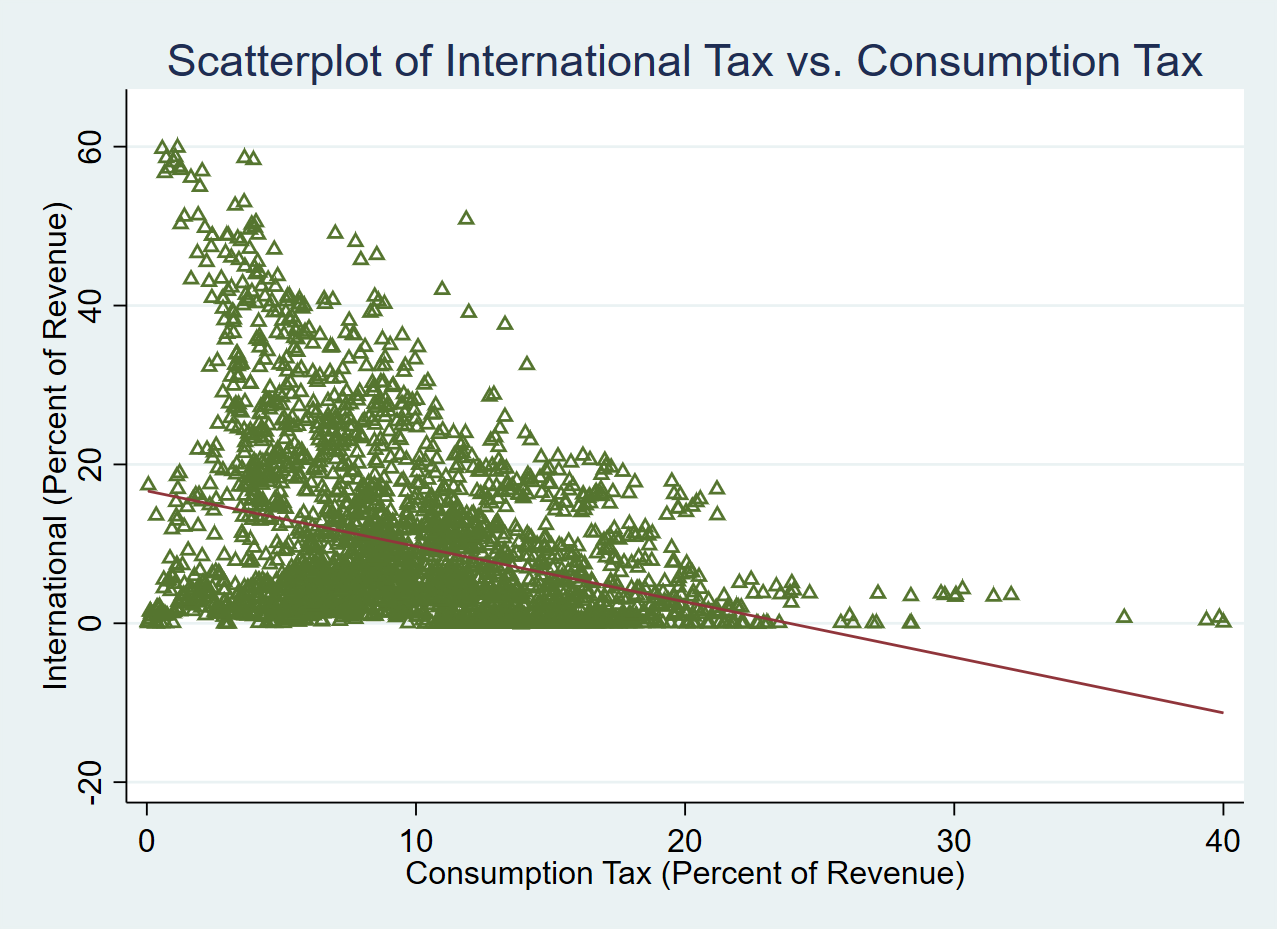
\includegraphics[width=0.8\linewidth]{Reproducibility_Package//research_outputs/Scatterplotintvscons.png}
    \caption{Scatterplot of International tax vs. Consumption Tax}
    \label{fig:enter-label}
\end{figure}

A graphical visualization of the whole data is best represented by Figure 4; a scatterplot including international and consumption data. A line of best fit is displayed on the graph, which has the same slope as the overall correlation for the data set at y=-0.3255. This reveals an inverse relationship between international and consumption tax variables. The data includes information from 194 countries from 1988 to 2022. The x-axis represents consumption tax and y-axis represents international tax, both in terms of percent of revenue. The line of best fit with a negative slope and negative correlation test indicate a moderate inverse relationship between these variables. 

With a pairwise correlation coefficient  of -.3255, the variables have a moderate strength negative correlation. A P-Value of 0.000 is a statistically significant value, meaning that the observed data is highly inconsistent with the null hypothesis giving us reason to reject the null hypothesis. This means there is a statistically significant relationship between tariffs and consumption taxes in developing and developed countries. However, rejection of the null hypothesis does not prove the alternative hypothesis true. Thus, we reject the null hypothesis that there is no relationship between these two variables. 

A significance test done on developing countries reveals a correlation coefficient of -0.3427, with a P-Value of 0.000 giving us further evidence to reject the null hypothesis. A significance test done on developed countries gives a correlation of coefficient of -0.2509, with a P-value of 0.000. Thus, we can confidently reject the null hypothesis and take note that the correlation between consumption tax and tariffs is weaker in developed countries than it is in developing countries. However, it must be noted that this result could be due to the higher amounts of data entries for developing countries. 

Additionally, we conducted a two sample T-test on the variable consumption by developed and developing countries, as well as another T-test on the variable international by developed and developing countries.

\begin{table}[H]
\centering
\caption{Two-sample t test International Tax Developed vs. Developing}
\label{tab:ttest_updated}
\renewcommand{\arraystretch}{1.2} % Adjust row spacing
\begin{tabular}{|l|r|r|r|r|r|r|}
\hline
\textbf{Group} & \textbf{Obs} & \textbf{Mean} & \textbf{Std. Err.} & \textbf{Std. Dev.} & \textbf{Variance} & \textbf{[95\% Conf. Interval]} \\ \hline
1              & 741          & 3.835927      & 0.3213594          & 8.747825          & 76.5075          & 3.205042 to 4.466811           \\ \hline
2              & 2,228        & 12.37055      & 0.2471915          & 11.66786          & 136.1931         & 11.8858 to 12.8553             \\ \hline
Combined       & 2,969        & 10.24049      & 0.2131389          & 11.61363          & 134.8826         & 9.822573 to 10.6584            \\ \hline
\textbf{Diff}  & \textbf{-}   & \textbf{-8.534625} & \textbf{0.466999} & -                  & -               & \textbf{-9.450299 to -7.61895} \\ \hline
\end{tabular}
\end{table}


% Table 2: Hypotheses Testing Results with Lines and Columns
\centering
\caption{Hypotheses Testing Results International Developed vs. Developing}
\label{tab:hypothesis_test}
\renewcommand{\arraystretch}{1.2} % Adjust row spacing
\begin{tabular}{|l|l|l|l|}
\hline
\textbf{Hypothesis}          & \textbf{Direction} & \textbf{p-value}      & \textbf{Result}       \\ \hline
$H_0$: diff = 0              & Equality           & -                     & Null Hypothesis       \\ \hline
$H_a$: diff $<$ 0            & Left-tailed        & $Pr(T < t) = 0.0000$  & Reject $H_0$          \\ \hline
$H_a$: diff $\neq$ 0         & Two-tailed         & $Pr(|T| > |t|) = 0.0000$ & Reject $H_0$       \\ \hline
$H_a$: diff $>$ 0            & Right-tailed       & $Pr(T > t) = 1.0000$  & Reject $H_0$          \\ \hline
\textbf{t-statistic}         & \textbf{-18.2755}  &                       &                       \\ \hline
\textbf{Degrees of Freedom}  & \textbf{2967}      &                       &                       \\ \hline
\end{tabular}

\bigskip

This T-Test table shows the T-test for the international variable against developed and developing countries. The purpose of the T-Test is to show if the means of developed and developing countries for international tax are statistically different from each other. The T-statistic value of -18.27 means that Group 1's mean is lower than Group 2's mean. This means that developed countries mean is lower than developing countries for the variable International Tax. This lines up with the findings of the histogram figures, summary statistics, and the  Michael. et. al (1993) readings which also reveal that Developed countries rely less on tariffs for revenue. Furthermore, all tests confirm the rejection of the null hypothesis, lending more credibility to the findings of our study and the potential that our alternative hypothesis could be true, subject to further testing. 

\begin{table}[H]
\centering
\caption{Two-sample t test Consumption Tax Developed vs Developing}
\label{tab:ttest_equal_variances}
\renewcommand{\arraystretch}{1.2} % Adjust row spacing
\begin{tabular}{|l|r|r|r|r|r|}
\hline
\textbf{Group} & \textbf{Obs} & \textbf{Mean} & \textbf{Std. Err.} & \textbf{Std. Dev.} & \textbf{[95\% Conf. Interval]} \\ \hline
1              & 1,100        & 11.61037      & 0.1728236          & 5.731912          & 11.27127 to 11.94947           \\ \hline
2              & 2,111        & 9.552993      & 0.1063205          & 4.88496           & 9.344489 to 9.761497           \\ \hline
Combined       & 3,211        & 10.25779      & 0.0931934          & 5.280867          & 10.07507 to 10.44052           \\ \hline
\textbf{Diff}  & -            & \textbf{2.057379} & \textbf{0.1930179} & -                 & \textbf{1.678928 to 2.435829}  \\ \hline
\end{tabular}
\end{table}



\begin{table}[H]
\centering
\caption{Hypotheses Testing Results Consumption Tax Developed vs. Developing}
\label{tab:hypothesis_test_results}
\renewcommand{\arraystretch}{1.2} % Adjust row spacing
\begin{tabular}{|l|l|l|l|}
\hline
\textbf{Hypothesis}          & \textbf{Direction} & \textbf{p-value}      & \textbf{Result}        \\ \hline
$H_0$: diff = 0              & Equality           & -                     & Null Hypothesis        \\ \hline
$H_a$: diff $<$ 0            & Left-tailed        & $Pr(T < t) = 1.0000$  & Reject $H_0$           \\ \hline
$H_a$: diff $\neq$ 0         & Two-tailed         & $Pr(|T| > |t|) = 0.0000$ & Reject $H_0$        \\ \hline
$H_a$: diff $>$ 0            & Right-tailed       & $Pr(T > t) = 0.0000$  & Reject $H_0$           \\ \hline
\textbf{t-statistic}         & \textbf{10.6590}   &                       &                        \\ \hline
\textbf{Degrees of Freedom}  & \textbf{3209}      &                       &                        \\ \hline
\end{tabular}
\end{table}

This Two sample T-Test shows a T-test for Consumption tax for developed and developing countries. It measures if the means of developed and developing countries for consumption tax are statistically significant. The T-statistic of 10.65 means the mean of Group 1 is higher than the mean of group 2. This reveals that Developing countries have a higher mean than developing countries for consumption tax. This lines up with the findings of the summary statistics, the visualizations from the two way histograms, and the Michael et. al (2003) readings. The P-value of 0.0000, gives us statistically significant evidence to reject the null hypothesis. 


\section{Conclusion}
\label{sec:conclusion}

In this study, we examined the relationship between consumption taxes and tariff revenue in developing countries, aiming to determine if there is an inverse relationship between these two forms of taxation. By analyzing data from the World Integrated Trade Solution (WITS) database spanning from 1988 to 2022, we found a moderate negative correlation between VAT revenue and tariff revenue across 194 countries. This suggests that if Value Added Tax increases, tariffs will decrease and vice-versa. The correlation is weaker in developed countries and will need further testing against the correlation coefficient in developing countries to find out if this difference is statistically significant. 

Overall, running a P-value test reveals the negative correlation between consumption taxes and international taxes, with a statistically significant P-value of 0.000. As a result, we reject the null hypothesis that an increase in Value Added Tax has no effect on International tax in developed or developing countries. The findings of our research show that both developed and developing countries have an inverse correlation in the data, most likely due to the fact that as countries develop they rely less on tariffs and more on value added tax. (Michael et. al 1993). 

While our study provides valuable insights into the relationship between consumption tax and tariff revenue in developing countries, several limitations must be acknowledged. One key issue is the quality and completeness of the data. Although the World Integrated Trade Solution (WITS) database is a robust source, the accuracy of data collection can vary across countries, particularly in developed nations where reporting practices may be inconsistent or incomplete due to the database sourcing most data from the UN Comtrade which has more data entries for developing countries. Missing or unreliable data could affect the relevance of our findings and introduce potential biases, especially when analyzing specific countries. 

While the overall trend and correlation indicate a clear relationship between consumption taxes like VAT and tariffs, there are several areas that warrant further investigation. Two particular things that we would like to look further into is country and regional level analysis. 

In the future, further analysis and research can be conducted at the country level, where time-series graphs can be generated, showing the change in consumption and tariffs over time. This would be particularly interesting for countries such as Brazil, India, and Ghana which have unique value-added taxation systems compared to other countries. Furthermore, this would enable analysis on countries which do not follow the negative correlation to be investigated, identifying particular reasons as to why this phenomenon occurs and observing if it aligns with the readings of Waglé (2011) and Bird (2008).  For example, countries with significant fluctuations in trade policy such as trade liberalization or protectionist measures could provide insights into how these changes affect the relationship between consumption-based taxes and tariffs. 

In addition, breaking down the data into regions or continents could shed light on whether the inverse relationship holds for different geographical areas or if regional differences play a role in the strength of this relationship. For example, could areas rich in natural resources have higher tariffs due to other countries demands for their resources? How would this effect value added tax? 

Overall, this research provides valuable insights for policymakers in developing countries. However, careful attention must be paid to the specific challenges each country faces, particularly in enforcing consumption taxes and addressing the circumstances of their specific economy. Future research should focus on further refining these findings and exploring the political and regional factors that may shape the relationship between consumption taxes and tariffs.

Lastly, we would like to thank Professor Buzard for the opportunity to complete this research report in her class, along with the valuable skills she has taught us in research report and drafting as well as stata analysis. We would like to thank Professor Ly for creating the research question on which this paper is based as well. 

\newpage
\section*{Bibliography}
\singlespacing
\setlength\bibsep{0pt}

Michael, Michael S., Panos Hatzipanayotou, and Stephen M. Miller. "Integrated reforms of tariffs and consumption taxes." Journal of Public Economics 52.3 (1993): 417-428.

Hansen, John Mark. “Taxation and the Political Economy of the Tariff.” International Organization 44.4 (1990): 527–551.

Waglé, Swarnim. "Coordinating tax reforms in the poorest countries: Can lost tariffs be recouped?." World Bank Policy Research Working Paper 5919 (2011).

Ho, Thuy Tien, Xuan Hang Tran, and Quang Khai Nguyen. "Tax revenue-economic growth relationship and the role of trade openness in developing countries." Cogent Business and Management 10(2) (2023)

M. Shahe Emran, Joseph E. Stiglitz, "On selective indirect tax reform in developing countries" Journal of Public Economics 599-623 (2005)

Kowalski, P. (2005), "Impact of Changes in Tariffs on Developing Countries' Government Revenue", OECD Trade Policy Papers, No. 18, OECD Publishing, Paris

Freed, Jeffrey S, et al. “Which Country Is Truly Developed? Covid-19 Has Answered the Question.” Annals of Global Health, U.S. National Library of Medicine, 18 May 2020

Bird, Richard M. (2008), "Tax Challenges Facing Developing Countries" Institute for International Business Working Paper No. 9

Liu Zhenmin, et al. "World Economic Situation and Prospects" United Nations Department of Economic and Social Affairs

United Nations. (2024) "Human Development Insights Database" Human Development Reports Data Center

PriceWater-HouseCoopers. (2024) "Value Added Tax Rates" Worldwide Tax Summaries 

United States International Trade Commission. (2024) "Harmonized Tariff Schedule 2024 HTS Revision 10" United States Government

World Integrated Trade Solutions (2024). "UN Comtrade" Frequently Asked Questions

United Nations (2024). "UN Comtrade Database" United Nations Department of Economic and Social Affairs

Marples, Donald J, "Consumption Taxes: An Overview" Congressional Research Service, January 24, 2023

International Monetary Fund Staff, "Global Trade Liberalization and the Developing Countries" International Monetary Fund

\newpage
\section*{Data Appendix} \label{sec:appendixa}
\addcontentsline{toc}{section}{Appendix A}

The Data Appendix is used to direct all readers to our \href{https://github.com/ecn310/course-project-taxes-tariffs/blob/main/Reproducibility_Package/README.md}{reproducibility package}. Our reproducibility package contains all of our raw data, modified datasets, do-files for complete statistical analysis, as well as do-files to generate all tables and graphs mentioned in this report. All do-files are commented on each line of code thoroughly explaining the process and methodology in order to get to the final results. 

\end{document}
